\documentclass[12pt]{article}
\usepackage[left=2cm,right=2cm,top=2cm,bottom=2cm,bindingoffset=0cm]{geometry}
\usepackage{fontspec}
\usepackage{polyglossia}
\usepackage{amssymb}
\setdefaultlanguage{russian}
\setmainfont[Mapping=tex-text]{CMU Serif}

\begin{document}
\centering {\LARGE Формальные языки}

{\Large домашнее задание до 23:59 24.09}
\bigskip

\enumerate
{
  \item Найти описание лексического синтаксиса вашего второго самого любимого языка программирования. В нем найти описание следующих языков:  
  \begin{itemize} 
      \item язык идентификаторов;
      \item язык ключевых слов (можно какого-нибудь их конечного подмножества);
      \item язык каких-нибудь чисел (целых в десятичной счисления, с плавающей точкой, любых других).
  \end{itemize}
    Для каждого из языков построить: регулярное выражение, недетерминированный конечный автомат, минимальный детерминированный конечный автомат. В отчете помимо этого указать ссылку на описание лекческого синтаксиса.
  \item 
  {
    Реализовать алгоритм Томпсона детерминизации конечных автоматов. 
        \begin{itemize}
        \item Сделать консольное  приложение, принимающее на вход путь к файлу, содержащему описание конечного автомата, производящее минимизацию и печатающее его результат в файл.
        \begin{itemize}
            \item Результатом работы минимизации является минимальный эквивалентный данному конечный автомат. Если автомат уже минимален, минимизация его не изменяет.
        \end{itemize}
        \item Составить набор тестов, демонстрирующий правильность работы реализации (качество тестового покрытия важно!).
        \item Код должен быть размещен на гитхабе, собираться одним скриптом, содержать инструкцию по сборке и запуску собранного приложения, собираться на чистой Ubuntu 18.04 или Windows 10. Все зависимости, в случае их отсутствия в системе, должны доставляться скриптом.
        \begin{itemize}
            \item Инструкция по запуску должна содержать информацию о том, где находится бинарник, как именно его полагается запускать, какой формат описания автомата, куда пишется результат.
            \item Можно писать на любом языке программирования. 
        \end{itemize} 
     \end{itemize}
  }

\newpage

\begin{center} \Large{Пример применения алгоритма Томпсона}
\end{center}

\bigskip

Детерминизируем данный автомат: 

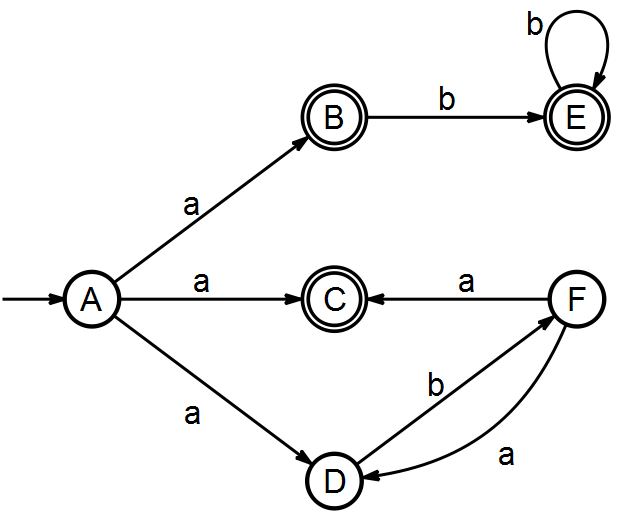
\includegraphics[width=0.65\linewidth]{../../2016_win/ElTech/2exdet.png}

Начинаем со стартового состояния. $\delta(A, a) = \{B, C, D\}; \delta(A, b) = \emptyset$. Добавляем вершину $\{B, C, D\}$, смотрим на переходы из нее: $\delta(B, b) = \{E\}; \delta(C, b) = \emptyset; \delta(D, b) = \{ F\}$. Объединяем результаты, получаем новое состояние $\{ E, F\}$ и переход $\delta'(\{B,C,D\}, b) = \{E, F\}$. Повторяем процедуру, пока не исследуем все переходы. Стартовое состояние --- множество из одного стартового состояния; терминальные состояния --- те, в которые попало хотя бы одно терминальное состояние исходного НКА.

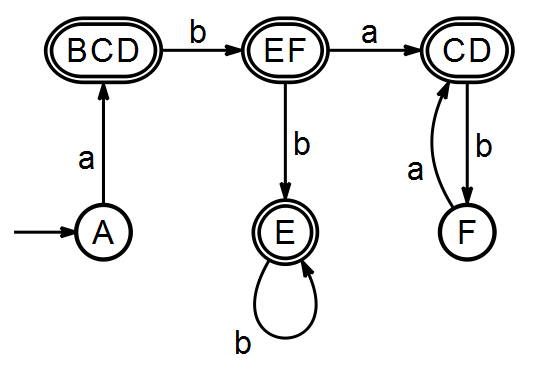
\includegraphics[width=0.65\linewidth]{../../2016_win/ElTech/2exdetres.png}

}

\end{document}